\chapter{Tools und Bibliotheken}

In diesem Kapitel werden Bibliotheken und Programme untersucht, die für das Projekt verwendet werden können. 
 
\section{Unterteilungsalgorithmen und Datenstrukturen}

Im Bereich Unterteilungsalgorithmen gibt es viele bereits implementierte Datenstrukturen und Algorithmen.
Gesucht wird eine einfache Datenstruktur, um Polygonnetze verarbeiten zu können.
Diese sollte so wenig Overhead wie möglich mitbringen.
Im Allgemeinen besteht solch eine Datenstruktur aus Ecken (Vertices), Kanten (Edges) und Flächen (Faces).
Zusätzlich muss noch die Beziehung zwischen den Objekten abgespeichert werden.

\subsection{OpenMesh}

OpenMesh wird von der \acs{RWTH} Aachen entwickelt und stellt eine mächtige Datenstruktur für Polygonnetze bereit.
Es steht unter der \acs{LGPL} v3 Lizenz (\enquote{with exception}) und kann somit problemlos verwendet werden.

OpenMesh implementiert eine Datenstruktur für Polygonnetze.
Darüber hinaus sind bereits einige Subdivision Algorithmen implementiert, die auf der OpenMesh Datenstruktur arbeiten können.
Zum Funktionsumfang gehören folgende Algorithmen.
\begin{enumerate}
\item Uniform subdivision
\begin{itemize}
	\item Loop
	\item Sqrt3
	\item Modified Butterfly
	\item Interpolating Sqrt3
	\item Composite
	\item Catmull Clark
\end{itemize}
\item Adaptive subdivision
\begin{itemize}
	\item Adaptive Composite
\end{itemize}
\item Simple subdivision
\begin{itemize}
	\item Longest Edge
\end{itemize}
\end{enumerate}

OpenMesh implementiert eine \emph{halfedge} Datenstruktur.
Diese \emph{edge-based} Datenstrukturen speichern die Information über die Verbindungen zwischen Eckpunkten (Vertices) in den Kanten (Edges), während
\emph{face-based} Datenstrukturen die Verbindungsinformation zwischen den Eckpunkten und Nachbarn in den Flächen (Face) speichern.\\
Jede Kante (Edge) referenziert also folgende Objekte:
\begin{itemize}
	\item 2 Eckpunkte (Vertices)
	\item eine Fläche (Face)
	\item die nächsten zwei Kanten (Edges) der Fläche
\end{itemize}

Halfedge bedeutet nun, dass eine Kante in 2 Halbkanten (Halfedge) aufgeteilt wird. Jede Halbkante hat nur eine Richtung.
Zwei Ecken A und B sind also über 2 Halbkanten (erste Halkante von A nach B und zweite Halbkante von B nach A) miteinander verbunden.
Dies bringt den Vorteil, dass man über die Kanten einer Fläche sehr einfach iterieren kann. Man muss dazu lediglich den Halbkanten folgen.


\subsubsection{OpenFlipper}

Aufbauend auf OpenMesh wurde von der \acs{RWTH} Aachen zusätzlich das flexible pluginbasierte Framework OpenFlipper enwickelt.
Damit können geometrische Objekte modelliert und verarbeitet werden. Intern wird auf die Datenstrukur OpenMesh zurückgegriffen.
Für die grafische Oberfläche wird QT verwendet.
Mit OpenFlipper kann man über die Oberfläche Netze erstellen und die in OpenMesh implementierten Subdivision Algorithmen anwenden.
\autoref{fig:openflipper} zeigt die Benutzeroberfläche von OpenFlipper.
\begin{figure}
  \caption{OpenFlipper}
  \centering
  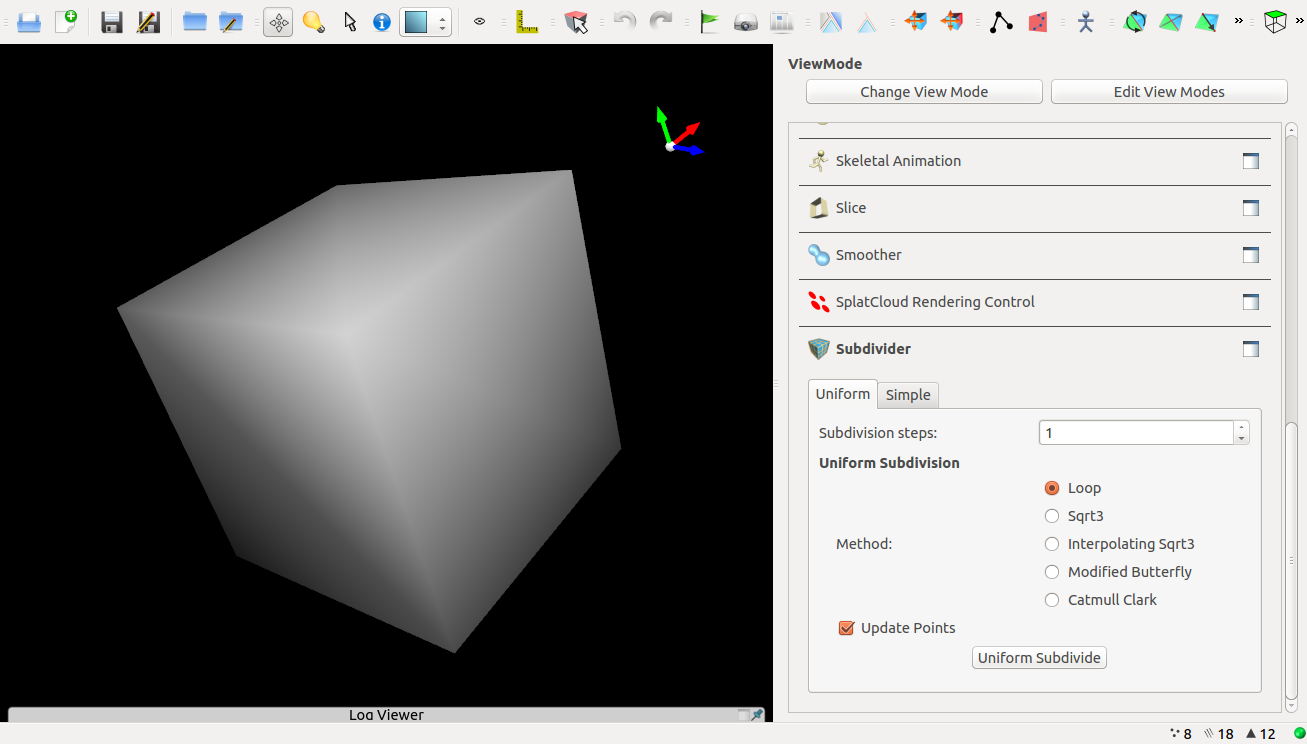
\includegraphics[width=0.8\textwidth]{content/media/openflipper_cube}
  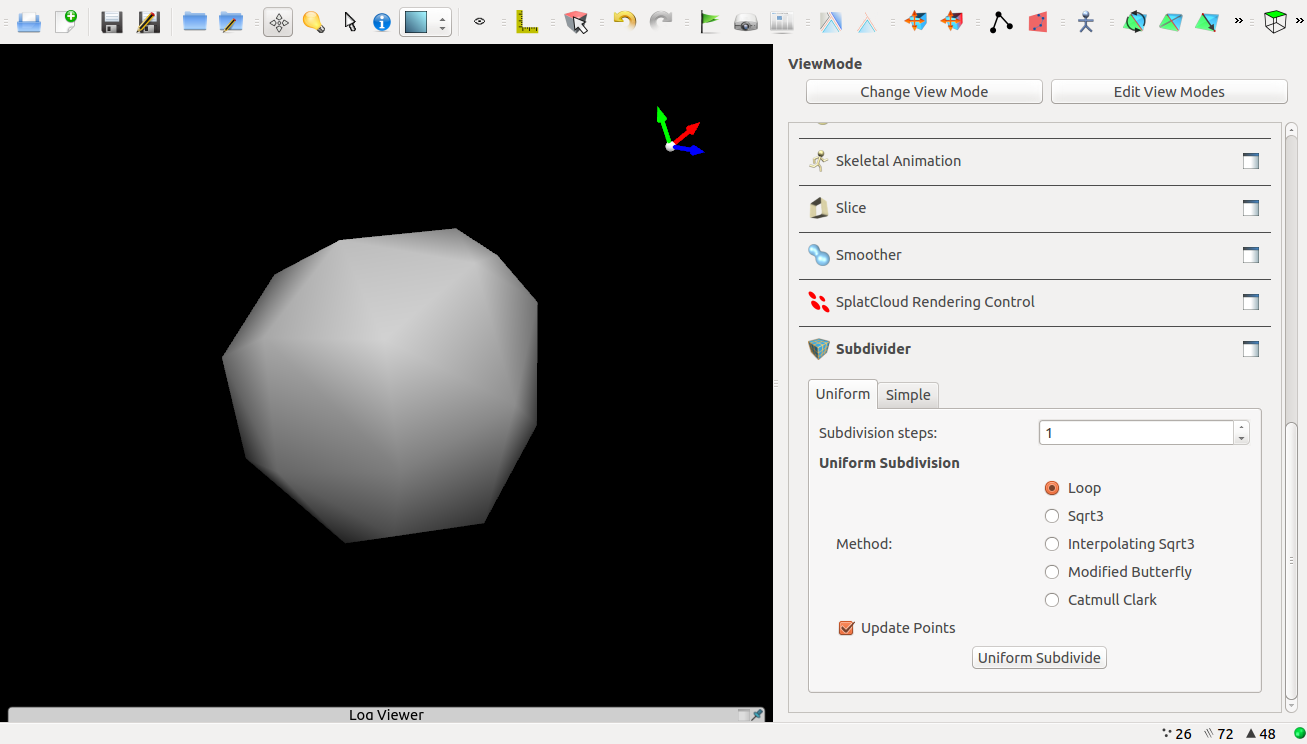
\includegraphics[width=0.8\textwidth]{content/media/openflipper_loop}
  \label{fig:openflipper}
\end{figure}


\subsection{Surface\_mesh}

Surface\_mesh ist eine einfache und effizente Datenstruktur um Polygonnetze beschreiben zu können.
Die Datenstruktur wurde alse einfachere Alternative zu OpenMesh von der Bielefeld Graphics \& Geometry Group entwickelt.
Die Datenstruktur soll einfach zu benutzen sein und eine bessere Performance und geringeren Speicherverbrauch mitbringen.
Analog zu OpenMesh implementiert Surface\_mesh eine halfedge Datenstruktur.
Die Verbindungsinformation der Kanten werden also in einem Paar aus zwei gerichteten Halbkanten gespeichert.
\autoref{fig:sm_halfedge} visualisiert den Zusammenhang der Halbkanten und Ecken.

\begin{figure}
  \caption{Surface\_mesh - Halfedge Verbindungen}
  \centering
  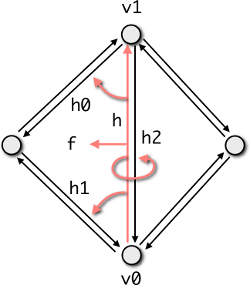
\includegraphics[width=0.3\textwidth]{content/media/sm_connectivity-queries}
  \label{fig:sm_halfedge}
\end{figure}

Da Surface\_mesh auch als Halfedge Datenstruktur implementiert ist, kann ähnlich effizient zu OpenMesh über die Kanten iteriert werden.
\autoref{lst:sm_iterate} zeigt einige Basisoperiation, die möglich sind.
Die Operationen aus Listing~\ref{lst:sm_iterate} sind zum besseren Verständnis in \autoref{fig:sm_halfedge} gekennzeichnet \cite{OpenGP.24.07.2015}. 

\begin{lstlisting}[style=myCppStyle, caption=Surface\_mesh - Basisoperationen, label=lst:sm_iterate]
Surface_mesh::Halfedge h;
Surface_mesh::Halfedge h0 = mesh.next_halfedge_handle(h);
Surface_mesh::Halfedge h1 = mesh.prev_halfedge_handle(h);
Surface_mesh::Halfedge h2 = mesh.opposite_halfedge_handle(h);
Surface_mesh::Face     f  = mesh.face_handle(h);
Surface_mesh::Vertex   v0 = mesh.from_vertex_handle(h);
Surface_mesh::Vertex   v1 = mesh.to_vertex_handle(h);
\end{lstlisting}

Um das Netz zu verändern oder zu editieren unterstützt die Datenstruktur high-level Operationen zum Verändern der Topologie.
Mit \emph{Edge Collapse}, \emph{Edge Split} und \emph{Edge Flip} kann das Netz geändert werden.
Die Operationen sind in \autoref{fig:sm_topology} dargestellt \cite{OpenGP.24.07.2015}. 

\begin{figure}
  \caption{Surface\_mesh - High-level Operationen zum Ändern der Topologie}
  \centering
  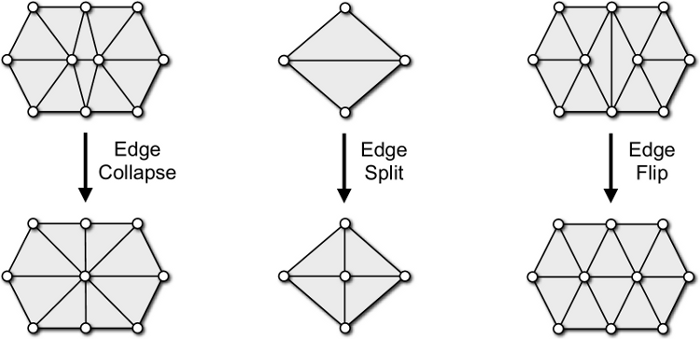
\includegraphics[width=0.8\textwidth]{content/media/sm_topology-changes}
  \label{fig:sm_topology}
\end{figure}

\subsection{OpenSubdiv}

OpenSubdiv wird von Pixar entwickelt und ist eine mächtige Bibliothek, die Subdivision Algorithmen und Datenstrukturen implementiert.
Die Bibliothek ist optimiert auf Performance und unterstützt paralleles Rechnen auf CPU und GPU.
Primär wird die Bibliothek von Pixar zum erstellen von animierten Filmen verwendet.
OpenSubdiv ist lizensiert unter der Apache License und darf somit frei für kommerzielle und nicht kommerzielle Projekt genutzt werden.

\begin{figure}
  \caption{Pixar OpenSubdiv Architektur \cite{Pixar.27.07.2015}}
  \centering
  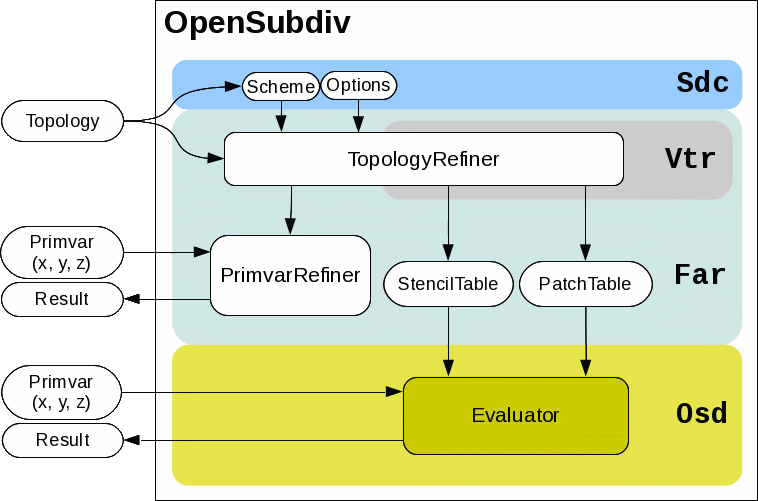
\includegraphics[width=0.9\textwidth]{content/media/pixar_opensubdiv}
  \label{fig:pixar_opensubdiv}
\end{figure}

\autoref{fig:pixar_opensubdiv} zeigt den Aufbau der OpenSubdiv Bibliothek.
Sie besteht insgesamt aus den 4 Schichten \ac{Sdc}, \ac{Vtr}, \ac{Far} und \ac{Osd} \cite{Pixar.27.07.2015}.

\begin{description}
 \item[\acs{Sdc}] ist der unterste Layer in der Architektur und implementiert die konkreten Subdivision Details.
 Dazu gehören Typen, Optionen und Eigenschaften für die konkreten Subdivision Algorithmen.
 \item[\acs{Vtr}] beinhaltet Klassen, die das Netz für effiziente Verfeinerung in einer Zwischenrepresentation darstellen.
 Diese Schicht ist nur für den internen Gebrauch gedacht.
 \item[\acs{Far}] ist die zentrale Schnittstelle, um Netze mit Subdivision Algorithmen zu verarbeiten.
 \item[\acs{Osd}] beinhaltet geräteabhängigen Code, um Objekte aus der Schicht \acs{Far} auch in unterschiedlichen Backends wie
 \acs{CUDA} oder OpenCL ausführbar zu machen.
\end{description}

Von OpenSubdiv werden die Subdivision Algorithmen \emph{Catmull-Clark}, \emph{Loop} und \emph{Bilinear} unterstützt \cite{Pixar.27.07.2015}. 

\subsection{CGoGN}

CGoGN ist eine Geometric Modeling C++ Bibliothek und implementiert eine Datenstruktur für n-dimensionale Netze als Combinatorial Maps.
Diese Implementierung unterscheidet sich zu den halfedge Datenstrukteren von OpenMesh und Surface\_mesh deutlich.
Diese sind zwar alle effizient, haben jedoch Probleme beim Umgang mit Objekten von unterschiedlichen Dimensionen.
Für jeden Problemfall muss die spezielle Datenstruktur verwendet werden.
All diese Strukturen lassen sich jedoch auf Combinatorial Maps zurückführen.
Diesen allgemeineren Ansatz geht CGoGN.
CGoGN implementiert bereits den Subdivision Algorithmus Catmull-Clark \cite{CGoGN.27.07.2015}. 

\subsection{\acf{CGAL}}

\ac{CGAL} ist ein mächtiges Softwareprojekt mit einer Vielzahl an Datenstrukturen und Algorithmen.
Neben Subdivision Algorithmen werden auch eine Reihe anderer Themengebiete abgedeckt (Voronoi Diagramme, Convex Hull Algorithms, Spatial Searching ...).
Für die Representation von Netzen gibt es bei \acs{CGAL} mehrere Möglichkeiten.

\begin{description}
 \item[Surface\_mesh] Zum einen implementiert \acs{CGAL} die bereits vorgestellte Datenstruktur Surface\_mesh.
 \item[3D Polyhedral Surface] Neben Surface\_mesh kann auch die von \acs{CGAL} entwickelte halfedge Datenstruktur Polyhedral verwendet werden.
\end{description}

\acs{CGAL} ist sehr mächtig und komplex. Die Bibliothek ist sogar in den meisten Paketquellen der Linux Distributionen enthalten (Ubuntu ...)
und kann darüber sehr leicht installiert werden.
Es sind auch bereits die Subdivision Algorithmen \emph{Catmull-Clark}, \emph{Doo-Sabin}, \emph{Loop} und \emph{Sqrt3} implementiert \cite{CGAL.27.07.2015}.

\subsection{Vergleich}

\autoref{tab:sd_bib} gibt einen Überblick über die Vorgestellten Bibliotheken listet auf, welche der ausgewählten Subdivision Algorithmen
(Catmull-Clark, Loop, Butterfly und Doo-Sabin) bereits implementiert sind.

\begin{table}
\caption{Vergleich der Subdivision Bibliotheken}
\center
\begin{tabular}{l|c|c}
\textbf{Bibliothek} & \textbf{Datenstruktur} & \textbf{Subdivision}\\
\hline
\textbf{OpenMesh} & halfedge & Catmull-Clark, Loop, Butterfly\\
\textbf{Surface\_mesh} & halfedge & keine\\
\textbf{OpenSubdiv} & halfedge & Catmull-Clark, Loop\\
\textbf{CGoGN} & combinatorial maps & Catmull-Clark\\
\textbf{\acs{CGAL}} & halfedge & Catmull-Clark, Loop, Doo-Sabin\\
\end{tabular}
\label{tab:sd_bib}
\end{table}

Mit Außnahme von Surface\_mesh, das wirklich nur die Polygonnetz-Datenstruktur mit elementaren Algorithmen implementiert, sind bei den anderen Bibliotheken bereits
einige Subdivision Algorithmen implementiert.
Bei Verwendung von OpenMesh oder CGAL könnte man sich viel Arbeit, da dort schon fast alle gewünschten Algorithmen implementiert sind.
Ziel dieses Projektes ist jedoch eine einfache und schnelle Implementiertung der Algorithmen.
Surface\_mesh selbst besteht nur aus wenigen Dateien und ist die schlankste Bibliothek von allen vorgestellten.
\autoref{fig:surface_mesh_cmp} zeigt die Ergebnisse eines Benchmark-Vergleichs für die unterschiedlichen Datenstrukturen.
In dem Diagramm werden die Zeiten relativ zu Surface\_mesh angegeben.

\begin{figure}
  \caption{Design, Implementierung und Evaluierung von Surface\_mesh \cite{Sieger.}}
  \centering
  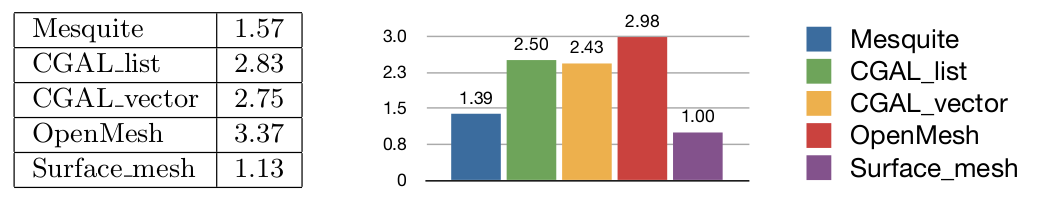
\includegraphics[width=1.0\textwidth]{content/media/surface_mesh_cmp}
  \label{fig:surface_mesh_cmp}
\end{figure}

Man erkennt deurlich, dass die Datenstrukturen von \acs{CGAL} und OpenMesh vergleichsweiße langsam sind.
Da Surface\_mesh sehr kompakt ist (es besteht nur aus sehr wenigen C++ und H-Dateien) und in dem Benchmark
auch sehr gute Ergnisse liefert, fällt die Wahl auf Surface\_mesh.


\section{Rendering}

Im folgenden Unterkapitel werden Bibliotheken oder Programme untersucht, die Polygonnetze rendern
und in wieweit diese Funktionen übernommen werden können. 

\subsection{BezierView}

BezierView (kurz bview) ist ein einfaches Programm zum Rendern von Bézier Patches, rationalen Bézier Patches und Polygonnetzen \cite{Peters.bview.27.07.2015}.
// TODO

\section{Grafische Oberfläche}

\subsection{QT}

// TODO

\subsection{libQGLViewer}

// TODO
